\chapter{Fundamentals on Integrated Sensing and Communication}
		
		% OLD PART
		%The fifth generation of cellular networks, with 5G New Radio (NR), introduced support for radio access technology-based localisation, an accurate positioning protocol and the ability to measure gaps on the NR carrier. 		This enables the system to estimate the positions of active user equipment (UE) by measuring time difference of arrival information \cite{Keating_Saily_Hulkkonen_Karjalainen_2019}.  The NR positioning protocol can also integrate satellite positioning systems and can be deployed as a private network solution with active user localization as described in  \cite{Henninger_Abrudan_Mandelli_Arnold_Saur_Kolmonen_Klein_Schlitter_Brink_2022}. The current standards, however, do not allow to detect passive devices, which refers to objects not directly connected to the network.
		
In recent years, research into cellular networks has focused on extending their capabilities, allowing them to do more than just transmit data.
Positioning of active \glspl{ue} was one of the first examples of these capabilities, defined in the \gls{3GPP} \Gls{lte} standard (Release 9).
\gls{lte} introduced support for positioning based on a wide range on methods.
These methods mostly rely on \gls{cid}, \gls{toa}, \gls{aoa}. Due to the accuracy requirements in different deployment conditions (\ie indoor or outdoor, urban or rural areas), \gls{lte} positioning normally employed two or more methods at the same time \cite{Razavi_Gunnarsson_2018}.
The fifth generation of cellular networks, with 5G \gls{NR}, expanded this capabilities. The introduction of beam-based operation and large antenna arrays, especially at mmWave, will enable higher positioning accuracy by exploiting more precise angular information in combination with time measurements \cite{Keating_Saily_Hulkkonen_Karjalainen_2019}.
Furthermore, the high available bandwidths will help in resolving multipath, thus facilitating correcting \gls{toa} estimation.
The \gls{NR} positioning protocol can also integrate satellite positioning systems and can be deployed as a private network solution with high accuracy indoor active user localization as described in  \cite{Henninger_Abrudan_Mandelli_Arnold_Saur_Kolmonen_Klein_Schlitter_Brink_2022}. 

The current standards, however, do not allow to detect passive devices, which refers to objects not directly connected to the network.
With the objective of expanding the capabilities of the mobile network, \gls{isac}, also known as JCAS or ICAS, is currently a topic of interest in the 6G research community \cite{Mandelli_Henninger_Bauhofer_Wild_2023}.
According to \cite{Viswanathan_Wild_2021}: "6G will function as a network with a \textit{sixth sense}". Radio signals transmitted by base stations, or users do not only carry data. They are affected by the movement of the transmitter or receiver, obstacles, movements of illuminated objects or changes in the propagation medium. Radio channels bear information about the environment in which the signal is transmitted. 
Channel information can, \eg, be obtained by removing the influence of the known, transmitted signal from the received one after target reflection. By analysing the channel response, it is possible to extract details about position, relative speed, type and shape of illuminated objects.

For 6G, the radio sensing capabilities should be integrated sharing the same spectrum for both communication and sensing purposes. Figure \ref{fig:isac-scheme-1} illustrates a fundamental sketch of an \gls{isac} scenario as described in \cite{Wild_Grudnitsky_Mandelli_Henninger_Guan_Schaich_2023}. In this depiction a cellular system is shown equipped with array antennas capable of beamforming, serving the dual purpose of sensing and facilitating high-rate, low-latency communication to multiple users.
\begin{figure}[H]
	\centering
	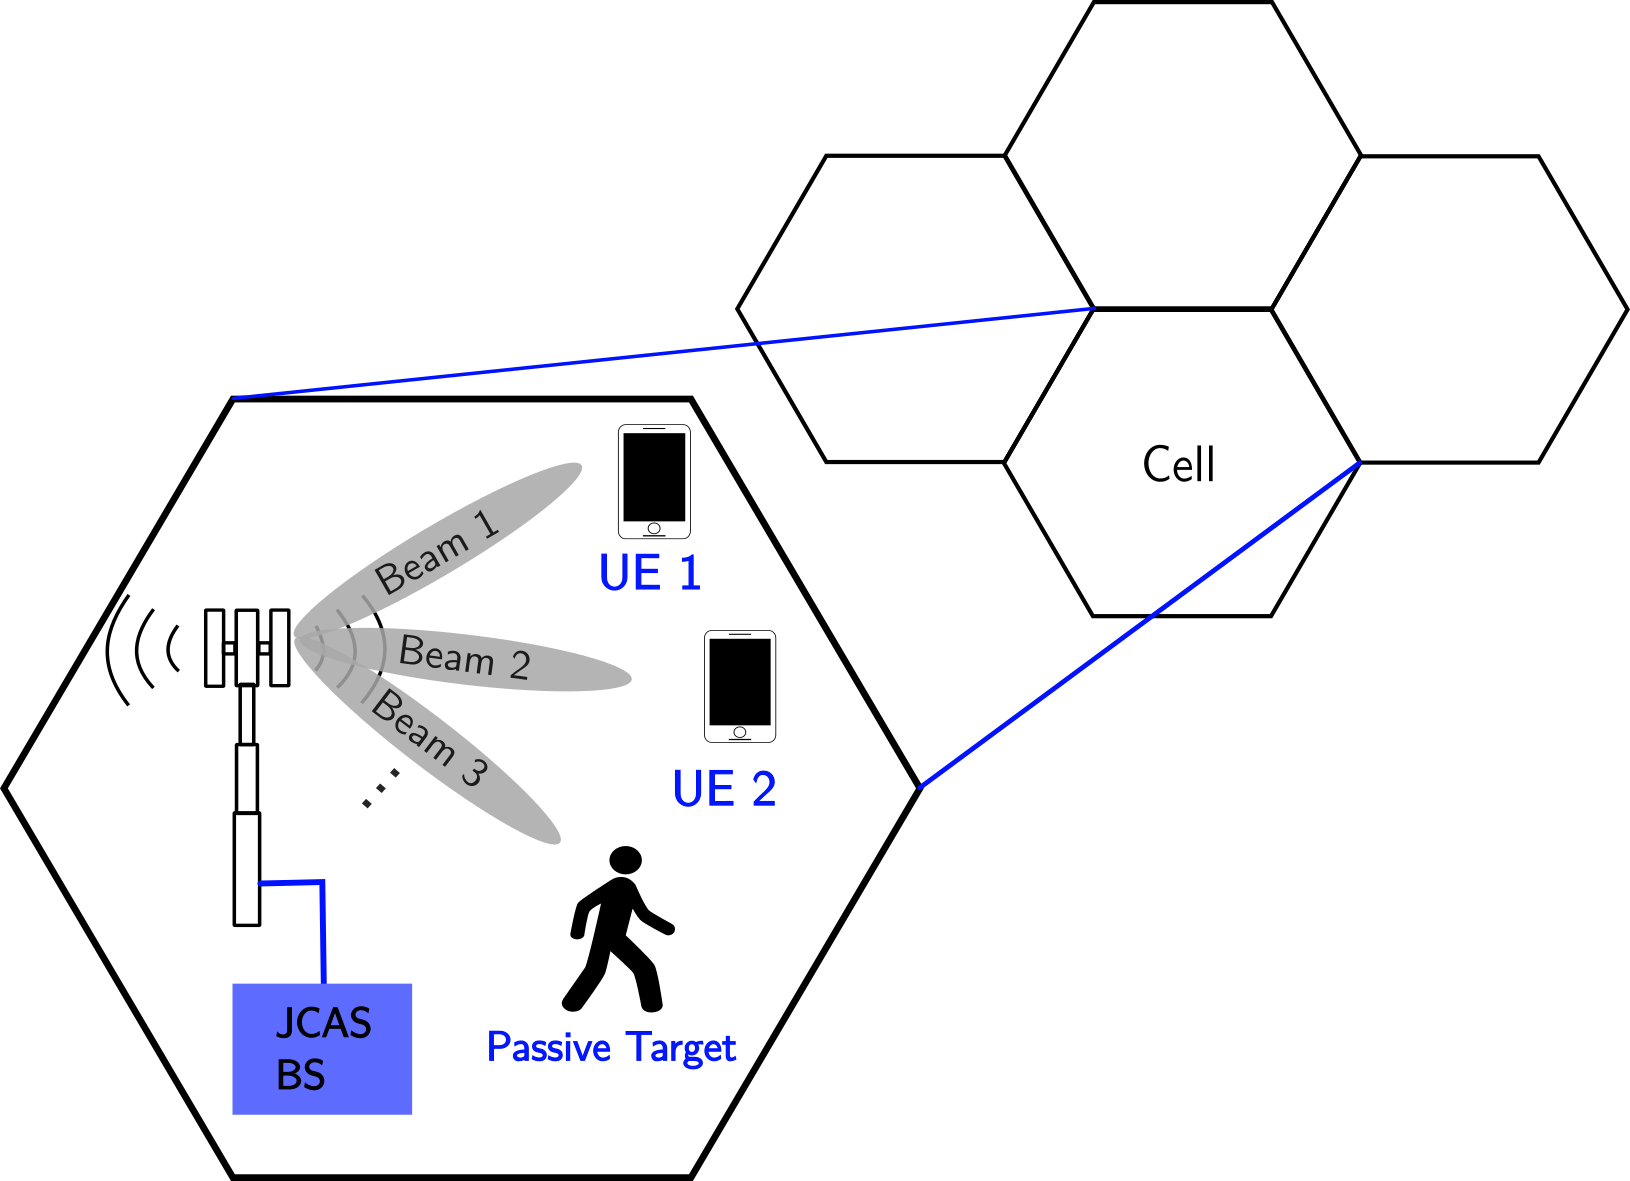
\includegraphics[width=0.8\textwidth]{Images/introduction/isac-scheme-1.png}
	\caption{Illustration of an \gls{isac} scenario.}
	\label{fig:isac-scheme-1}
\end{figure}
\Gls{isac} essentially aims at operating the network as a radar, while benefiting from the massive deployment of cellular networks and their coverage, making use of existing hardware and extending its capabilities with sensing.
The network will be able to adapt and use information about the surrounding environment, combined with active positioning of \glspl{ue}, as a source of situational knowledge.



\section{Technological enablers}

	This section will present some of the main technological aspects and digital technologies enabling joint sensing and communication and the current research on radar in communication systems.	
	
	\subsection{Spectrum choice for 6G sensing}

	One of the goals set for the sixth generation of wireless networks is to make efficient usage of the available spectrum which is one of the scarcest resource in communications.
	
	Future systems will probably make use of larger frequency bands, exploiting high bandwidth to perform high-resolution sensing. From 20 MHz carriers in LTE, to 100 MHz to 400 MHz in 5G NR and mmWave \gls{NR}, it can be expected that \gls{5G} evolution and 6G systems will use bandwidths in the order of 1 GHz or more. A large usable bandwidth will allow for increased range resolution for sensing.
	
	Spectrum choice will be the determining factor for the definition of overall capabilities of the system. The frequency ranges that are being considered for 6G \cite{Hexa} are:
	
	\begin{itemize}
		\item \Gls{fr1}: from 600 MHz to 6 GHz;
		\item \Gls{fr2}: mmWave, from 24 GHz to 71 GHz;
		\item the new \gls{fr3}, not yet specified: likely from 7 to 20 GHz
	\end{itemize}
	
	\Gls{fr1} is currently used for \Gls{5G} capacity layers, providing a bandwidth of up to 100 MHz. For 6G, the main capacity layer will be placed in the "Golden Band" in 6-14 GHz, offering up to 400 MHz of bandwidth. \Gls{fr2} in the millimetre frequency bands will start at 24 GHz and offer significantly more bandwidth, up to 1 GHz.
	
	\Gls{fr3} and \Gls{fr2} are the most relevant candidates for defining the sensing spectrum in 6G. Their selection would make sense for wide area sensing and high resolution sensing, respectively.
	
	Feasible use cases and possible scenarios will be driven by the characteristics and specifications offered by the frequency band of choice. It can be expected that \Gls{fr2} will be used in micro-cellular deployments. They will, \eg, be deployed in indoor environments, such as factory floors. Sensing targets in such environment will likely be pedestrians, passive factory objects and vehicles.
	Macro-cellular environments in the Golden Bands will dominate outdoors, where targets of interest will be vehicles for traffic monitoring, roadside safety and even detection of \gls{uav}, such as drones \cite{Mandelli_Henninger_Bauhofer_Wild_2023}.
	
	\subsection{Waveform candidates for ISAC}
	
	Waveform design is a fundamental building block of any radar or communication systems. Traditional radar and communication systems use waveforms optimized for the respective use, that are, in general, very different \cite{Zhang_Rahman_Wu_Huang_Guo_Chen_Yuan_2022}.
	
	In this work we refer to a communication-centric design, where the communication system is adapted and expanded in order to perform the sensing operation, sharing the main hardware and resources provided by the wireless mobile network.
	 
	
	\subsubsection{Traditional radar waveforms}
	
	Conventional radar systems mainly consist of pulsed and continuous wave radar. Both types can be further categorised according to whether the wave is modulated in frequency or phase \cite{Friedlander_2007}.
	Pulsed radar transmits short, typically unmodulated, pulses or bursts of pulses of large bandwidth, followed by a silent period, waiting for the reception of the echoed signal. Continuous wave radars are currently largely used in automotive systems and the main example are \gls{fmcw} radars. Such systems transmit chirp signals with fixed or variable frequencies, which get shifted by the so called beat frequency when they get reflected by objects.
	
	Radar systems are typically designed to enable high power transmission with a relatively simple receiver structure. Two of the main design objectives are amplifier efficiency and ideal autocorrelation properties of the radar wave. Waveforms with low \gls{papr} enable high efficiency and long range transmission.
	
	Due to their specialized signal shape and relatively simple hardware, these systems cannot support high data-rates for communication purposes, especially the ones that will be required by 6G.
	
	\subsubsection{Communication-centric waveforms}
	
	Current mobile communications are dominated by multi-carrier waveforms (\gls{ofdm}).
	\GLS{ofdm} has become the current waveform reference in \gls{isac}. Fully established as the standard in 4G and 5G communications systems, in the last decade it has also attracted the attention of the radar world.
	
	\gls{ofdm} offers great multiplexing capabilities, both in time and in frequency, through the definition \textit{OFDM resource elements} that can be dynamically allocated to users. The use of cyclic prefix transforms the linear convolution of the signal with the channel response into a circular convolution, allowing convenient equalisation of the channel in the frequency domain \cite{Wild_Grudnitsky_Mandelli_Henninger_Guan_Schaich_2023}. In scenarios limited by \gls{papr} constraints, such as uplink transmission, DFT spreading can  be applied on top of \gls{ofdm} to achieve a single-carrier frequency division multiple access (SC-FDMA) scheme.
	
	The idea of using OFDM for sensing purposed was first proposed in \cite{Levanon_ofdm} in 2000. One of the first proposal for signal processing for OFDM radar was developed by Strum and Wiesbeck in \cite{Sturm_Wiesbeck_2011}.
	\gls{ofdm} waveforms do not require the high autocorrelation characteristics that are normally expected from traditional radar waveforms, while being able to fulfil requirements for both communications and sensing performance.
	
	\subsubsection{Waveforms for next-gen communication networks}
	
	One of the major challenges for \gls{ofdm}, and multi-carrier waveforms in general, is the performance loss observed in particular environments characterized by highly frequency-dispersive channels (\eg high mobility scenarios, dynamic wireless networks).
	The effect of phase noise and movement (Doppler spread) is enhanced at high carrier frequencies. 
	Due to the expansion of 5G and 6G systems towards mmWave, tackling this challenge is fundamental for ensuring high performance under these circumstances.
	
	\Gls{otfs} has been proposed as a modulation effective in tackling these problems. \Gls{otfs} operates in the delay-Doppler domain. 
	The fading, time-variant channel seen by an \gls{otfs} signal is transformed into a non-fading, time-independent channel through a 2D Fourier transform \cite{OTFS_Hadani_2017}. 
	Applying this transformation and equalization within this domain each symbol will experience similar gain during transmission.
	
	\gls{otfs} can be interpreted as the sequence of two transformations. 
	Firstly, the transmitter maps the complex symbols into discrete slots in the delay-Doppler domain.
	Secondly, these symbols are transformed in the time-frequency domain through a 2D inverse symplectic finite Fourier transform (iSFFT). The the time-domain signal is obtained by using the \gls{ifft}. 
	The receiver will perform the inverse operation using \gls{fft} and SFFT, respectively.
	\gls{otfs} is an suitable waveform for integrating sensing and communication due to its inherent property of operating in the delay-Doppler domain.
	
	Although \gls{otfs} has proved to achieve some advantage compared to \gls{ofdm} in highly fading and mobility scenarios \cite{OTFS_Hadani_2017}, its implementation in real systems is hindered by some open research problems. 
	The primary challenge is to develop an efficient decoding method for \gls{otfs} symbols.
	The output signal in the delay-Doppler domain is a 2D circular convolution of the transmitted data symbols and the channel response. Although optimal detectors, such as \gls{map} detectors, can mitigate channel interference and perfectly retrieve the original symbols, they are too complex and costly \cite{Raviteja_Viterbo_OTFS_decoding}.
	
	This work will focus on \gls{ofdm}, as it is the waveform currently used in 5G systems and in the proof of concept by Nokia. 
	As the current standard \gls{ofdm} is well established with widely available hardware support, and has been able to provide high speed communications with high spectral efficiency and robustness to multipath and frequency-selective fading.
	Furthermore, \gls{ofdm} systems are able to perform simple channel equalization, by using the single-tap technique.
	
	 
	
	\subsection{5G functional splits}
	
	A functional split determines the number of functions implemented locally at the \gls{ru} and, consequently, the functions to be implemented in a centralised datacenter \cite{Larsen_Checko_Christiansen_2019}. 
 	This solution was developed to define a flexible approach to the \gls{cran} concept, that could work with the high data rates expected in 5G. 
	In \gls{NR}, the radio processing stack defined by \gls{3GPP} is split between a \gls{du} and a \gls{cu}. 
	The general idea is to keep functions close to the user in the \gls{du}, while placing more complex and computationally intensive functions in the \gls{cu}. The \gls{cu} is usually represented by powerful datacenters.
	Allocating more functions in the \gls{du} means less traffic on the fronthaul network, but requires more powerful and expensive hardware at the antenna site.
	Functional splits allow for a fairly flexible architecture of the system. Additional functionality, such as network sensing, can be implemented at the \gls{ru} by adding dedicated processing hardware.

	%\begin{figure}[H]
	%	\centering
	%	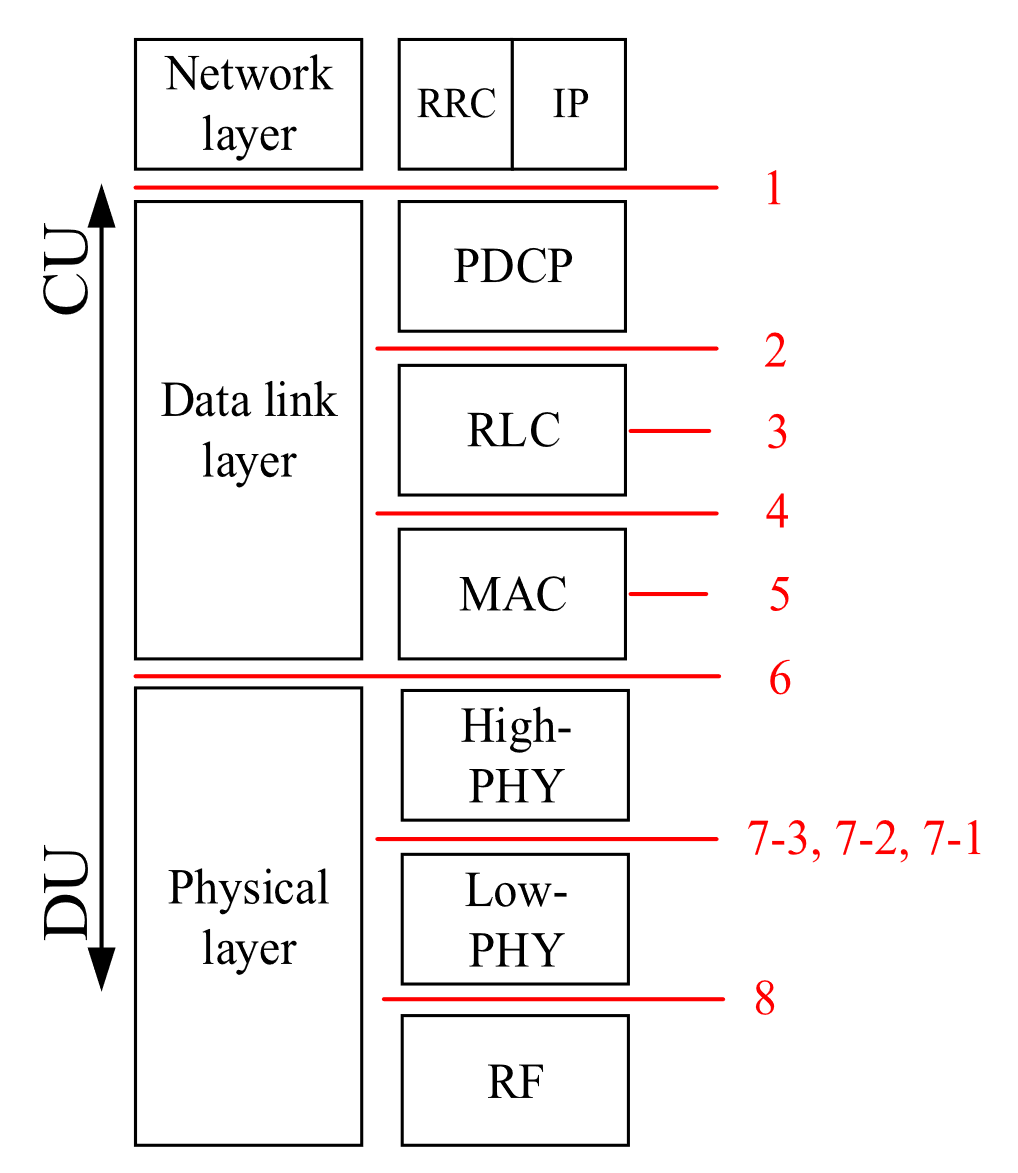
\includegraphics[width=0.5\textwidth]{Images/overview/5Gsplits_Larsen.png}
	%	\caption{Scheme representing the LTE protocol stack, showing proposed functional splits %\cite{Larsen_Checko_Christiansen_2019}. }
	%	\label{fig:Overview-LTE_stack_splits}
	%\end{figure}
	 
	
	\subsection{Massive MIMO and beamforming}
	
	Massive \gls{mimo} and digital beamforming can set the basis for performing high-resolution three-dimensional scans of the surrounding environment \cite{MIMO-next-gen}.
	The general idea is to intelligently combine the signals received from multiple antennas to achieve high signal-to-noise ratios and data rates.
	
	In \gls{5G}, beamforming commonly employs an all-digital approach at lower frequencies. However, for mmWave frequencies and above, analogue or hybrid beamforming is typically used. 
	
	Hybrid beamforming allows to scan multiple beams at the same time, controlled by $P >1$ RF chains, where $P < Q$ where $Q$ is the number of antennas. 
	The transmitting cells can perform a beam sweep, where the signal is steered over different angles. 
	Using beam sweeps for \gls{isac} allows to collect complete spatial information about the environment surrounding the cell.
	
	\subsection{Signal processing enhanced by AI/ML}
	Generally, radar returns provide additional information beyond the range-Doppler profile. 
	By analysing the channel information, it may be possible to extract target characteristics such as radar cross-section, micro-Doppler information, or the object's material or shape.
	This additional information can be used to solve a classification problem of objects and radar returns.
	
	Recent years have seen \gls{ai} and \gls{ml} emerging as a novel and powerful method for extracting and processing information effectively, often surpassing traditional methods.
	In the radar world \gls{ai} has been used to solve target classification problems. 
	\Gls{ai} systems can accurately differentiate between various targets, such as aircrafts, ships, and ground vehicles, based on their radar signatures \cite{survey_radar_AIML}. 
	\gls{ai}-powered radar systems can adapt and learn from new data, continuously improving their capabilities over time. 
	This technology could assist the development of autonomous radar systems capable of making independent decisions based on the classification results. 
	
	 Furthermore, artificial intelligence and machine learning have already been introduced in communication systems to optimize network resources, improve overall quality of service, solve optimization problems, and predict system load and traffic \cite{30_years_ai_survey}. 
	 By combining sensing capabilities with \gls{ai}, nodes could effortlessly integrate the physical and digital domains, giving the network situational capabilities.
	


\section{Proof of concept architecture}
	\label{sec:intro-PoCarchitecture}
	
	The architecture considered in this work is based on \gls{fr2} 5G commercially available communication hardware.
	The system consists in a mmWave \gls{gnb} \gls{ru}, extended by a dedicated \gls{ru} called \textit{Sniffer} and a server called \gls{spu}. 
	The sniffer is synchronized with the \gls{gnb} by the same synchronization source. 
	The \gls{spu} receives the complex IQ signal,  after \gls{fft} and removal of the \gls{cp}, as input for further sensing processing on a per-radio frame basis \cite{Wild_Grudnitsky_Mandelli_Henninger_Guan_Schaich_2023}.
	
	Using option 7-2 of the proposed 5G splits, it is possible to use the same type of \gls{ru} for both communication and sensing.
	Option 7-2 splits the network at the \gls{phy} level, which handles the conversion of digital data to the analogue radio signal in \gls{dl}, while doing the opposite in \gls{ul}.
	This split defines the \gls{fft}/\gls{ifft} performed in the \gls{ru}, while the frequency domain IQ is transported on the fronthaul.
	The \gls{gnb} \gls{ru} operates in \gls{tdd} mode, where \gls{ul} is separated from \gls{dl} by the allocation of different time slots in the same frequency band. 	
	The sniffer operates always in \gls{ul} mode, receiving both the signal transmitted by \glspl{ue} and the reflected signals. 
	
	This work considers a \gls{poc} deployment where the primary \gls{gnb} \gls{ru} and the sniffer are mounted in proximity and are co-located, allowing the system to behave as a monostatic radar. 
	The scope of this work does not cover the case of bistatic radar.
	
	The SPU processing chain for sensing is structured as follows:
	
	\begin{itemize}
		\item \textit{Reference and reflected signal reception}. Receive and process packets from \gls{gnb} and Sniffer. Each radio frame has dimension $N\times M$, where $N$ is the number of subcarriers and $M$ the number of \gls{ofdm} symbols.
		\item \textit{Channel computation}. Channel information is obtained by division of the received by the transmitted frames.
		\item \textit{Clutter removal}. Before every measurement, the channel of the corresponding scenario without targets is saved during a calibration step and, based on that, the clutter components are removed from the reflected signal at runtime.
		\item \textit{Periodogram computation}. The spectral response of the channel information is obtained by computing $N$ \glspl{fft} followed by $M$ \glspl{ifft} on the result. The response is then converted in a 2D range-Doppler map of the observed targets. 
		\item \textit{Peak extraction}. Identifying the peaks in the periodogram allows to retrieve the range-speed information of targets present on the scene.
		\item \textit{Target tracking}. A \gls{kf} can be used to track the detected targets. 
	\end{itemize} 
	A more detailed description on how the processing chain is structured,  based on \cite{Braun2014OFDMRA}, will be presented in Chapter \ref{chap:theoretical_OFDM}.
	
	
	The system specifications are indicated in table \ref{table:PoCparams}.
	They correspond to parameters for 5G \gls{NR} systems with the numerology $\mu=3$ specified in \cite{TS138211}. 
	
	\begin{table}[H]
		%\caption*{\textbf{Title of Table (optional)}}
		\centering 
		\begin{tabular}{|p{9em} c c |}
			\hline
			\rowcolor{bluepoli!40} % comment this line to remove the color
			\textbf{Parameter} & \textbf{Description} & \textbf{Value}  \T\B \\
			\hline \hline
			$\mu$ & 5G numerology & 3 \T\B \\
			$f_C$ & carrier frequency & 27.4 GHz \T\B \\
			$B$ & bandwidth & 200 MHz \T\B\\
			$\Delta_f$ & subcarrier spacing & 120 kHz  \T\B\\
			$T_S = 1/\Delta_f + T_{CP}$ & symbol time & 8.92 $\mu s$  \T\B\\
			$T_{CP}$ & cyclic prefix time & 0.59 $\mu s$  \T\B\\
			$N$ & number of subcarriers & 1584  \T\B\\
			$M$ & number of symbols & 1120  \B\\
			
			\hline
		\end{tabular}
		\\[10pt]
		\caption{List of system parameters from Nokia proof of concept installation.}
		\label{table:PoCparams}
	\end{table}
	
	The system is equipped with analog beamforming and measurements can be obtained using a fixed beam for both \gls{gnb} \gls{ru} and sniffer, chosen from a beam codebook.


\section{Sensing use-cases}

	Several use cases has been proposed \cite{Mandelli_Henninger_Bauhofer_Wild_2023}, \cite{Wang_Varshney_Gentile_Blandino_Chuang_Golmie_2022} and  key requirements for each application have been estimated in \cite{Wild_Braun_Viswanathan_2021}.
	In order to understand system requirements and research approaches, it is essential to define likely scenarios in which \gls{isac} systems will be deployed.
	
	\subsubsection{Automotive radar}
	
	Automotive radar is essential for new generations of cars and future autonomous driving vehicles.
	Communication capabilities are also necessary to establish vehicle networks for sharing information on the surrounding environment.
	Modern vehicles have evolved from simple means of transport to smart vehicles equipped with a variety of sensors and communication equipment.
	The market for \gls{v2x} networks has been growing significantly in recent years \cite{Liu_Masouros_2021}.
	This network requires high communication performance, throughput, and low latency, as well as precise positional information on surrounding objects.
	
	\gls{isac} is an ideal candidate to fulfil these requirements, enabling efficient use of the spectrum and enhancing the physical layer security of the \gls{v2x} network.
	
	\gls{isac} systems must be capable of performing tasks such as vehicle and traffic counting, collision avoidance, and pedestrian and animal detection.
	
	\subsubsection{Outside Drone Detection}
	
	Detection of \gls{uav} may be necessary in various deployment scenarios, including rooftops of buildings, airports, and open urban areas.
	
	\glspl{uav} are typically equipped with sensors, cameras, and radars for surveillance and monitoring. Additionally, \glspl{uav} are used to provide connectivity in hazardous or data-intensive environments.
	\gls{isac} systems are suitable for fulfilling communication requirements in \gls{uav} networks while being able to detect unwanted drones in a monitored area.
	
	\subsection{Human activities}
	
	\Gls{isac} for human activities detection could be applied for tracking a subject's physical movements, as well as monitoring vital signs for healthcare applications. 
	
	The capacity to perceive and interpret human activities can offer valuable insights and enable interventions that enhance quality of life, performance, and safety.
	
	Micro Doppler tracking and feature extraction, combined with machine learning, can help distinguish between targets or extract additional information about activity and human presence in the monitored area.
	
	One such use case is the monitoring of roadways and industrial floors to enhance safety. \Gls{isac} can exploit the deployed network equipment of smart factory floors. Potential hazards can be detected in real-time, allowing for accident prevention. 
	
	Another valuable application of \gls{isac} is crowd monitoring. 
	The system can analyse crowd movements, density and motion patterns. 
	Crowd flows can be monitored by \gls{isac} systems while respecting the privacy of the individuals, compared to standard camera systems, as the identity of the targets is not disclosed to the system supervisor and cannot be extracted through face recognition algorithms.

	
	\subsection{Non-line-of-sight sensing}
	
	
	
	The term \textit{line-of-sight} (LOS)  denotes the existence of a direct, unobstructed line of sight between the transmitter and the target. On the contrary, \textit{non-line-of-sight} (NLOS) denotes the condition in which the target is reached by the transmitted signal via one or multiple reflections on another entity. 
	Feasibility of monostatic \gls{isac} in \gls{nlos} environments is still a rather unexplored area of research, as commonly studied use cases assume the target to be in \gls{los} \cite{Gustaffson_NLOS_radar}.
	
	The main advantage of \gls{nlos} sensing is the possibility of performing "around the corner" detection, which is not feasible with traditional fixed camera or LIDAR systems. 
	Sensing targets moving behind an obstacle would be a powerful feature in use cases such as automotive radar and surveillance systems.
	
	As we can expect cellular networks operating in \gls{fr2} also to be deployed in indoor areas and factory floors, this work will focus on intrusion detection in industrial scenarios.
	Intrusion detection in \gls{nlos} on factory floors could represent a valuable addition, from a commercial point of view, for private cellular networks in smart industries.
	
	In addition, it has the potential to enhance cellular sensing systems in a cost-effective manner, making them a viable alternative to expensive ad hoc systems. This approach does not require the deployment of infrastructure or specialized equipment. 
	\gls{nlos} sensing could be an attractive option for industries seeking to enhance their surveillance or monitoring systems while optimizing resources.
	
	%\remove{Furthermore, it could unlock new use cases that have yet to be fully explored. In industrial environments, non-line-of-sight sensing technology has the potential to enhance safety protocols and improve accident prevention measures by detecting humans within obscured or complex settings. Additionally, intrusion detection systems could benefit from this technology as it may enable the identification of unauthorized access attempts even in hidden or non-obvious entry points.}
	
	

